\documentclass[11pt]{article}

% ====================================================
% PACKAGES
% ====================================================
\usepackage[margin=1in, headheight=13.6pt]{geometry}
\usepackage[T1]{fontenc}
\usepackage{lmodern}
\usepackage{microtype}
\usepackage{setspace}
% \usepackage{parskip}
\usepackage{tcolorbox}
\usepackage{amsmath, amssymb, mathtools}
\usepackage{siunitx}

\usepackage{graphicx}
\usepackage{float}
\usepackage{subcaption}

\usepackage{enumitem}
\usepackage{booktabs}

\usepackage{xcolor}
\usepackage{hyperref}

\usepackage{fancyhdr}
\usepackage{lastpage}

\usepackage{listings}
\usepackage{indentfirst}
\usepackage[justification=centering]{caption}
% \usepackage{algorithm}
% \usepackage{algpseudocode}
% \usepackage{algorithmic}

% \onehalfspacing%


\pagestyle{fancy}
\fancyhf{}
% Header Design
\lhead{\Assignment\ |\ \course}
\rhead{\Name\ |\ \today}
\cfoot{Page \thepage\ of~\pageref{LastPage}}

\usepackage{listings}
\usepackage{xcolor}

\lstset{
    language=Matlab,
    basicstyle=\ttfamily\small,
    keywordstyle=\color{blue},
    commentstyle=\color{gray},
    stringstyle=\color{orange},
    numbers=left,
    numberstyle=\tiny,
    stepnumber=1,
    numbersep=5pt,
    frame=single,
    breaklines=true,
    showstringspaces=false
}


\newcommand{\Name}{Arael Anaya}
\newcommand{\Assignment}{1.3 Deep Dive into a Robotic Mission}
\newcommand{\course}{Space Robotics}


\lstset{
    language=Matlab,
    basicstyle=\ttfamily\small,
    frame=single,
    breaklines=true,
    numbers=left,
    numberstyle=\tiny,
    tabsize=2
}

% makes the hyperlinks look good
\hypersetup{
    colorlinks,
    linkcolor={red!50!black},
    citecolor={blue!50!black},
    urlcolor={blue!80!black}
}

% \setlength{\parindent}{1em}
\usepackage{indentfirst}

\begin{document}

\section*{Mission Selection \& Relevance}
Perseverance represents what I find most interesting
in robotics: autonomous decision-making under tight real-world constraints. Control systems is the
part of the robotics stack I am most passionate about. It's actually what my current internship focuses on. Seeing
Perseverance's dual-computer architecture manage competing tasks in a communication-delayed,
resource-constrained environment makes the concepts I study feel real and impactful~\cite{science_robotics}. The rover's perception pipeline is also an area I am working to understand
more deeply, making the study of its sensors relevant to my own learning.

\section*{Mission Statement}
Mars has always been of great interest to humans due to the high likelihood of it at one point
holding life. It is the most likely candidate for human colonization and, as such, understanding
it is one of the top priorities for our future in space.

The Mars 2020 Perseverance rover was designed to traverse the harsh environments of Mars as it
attempted to discover signs of ancient microbial life~\cite{rover_components}. As the first leg of
NASA's Mars Sample Return campaign, it also laid the groundwork for returning scientifically
selected samples to Earth for analysis that no onboard instrument could replicate~\cite{mars2020_wiki}.

\section*{Mission Objectives}
The rover was equipped with a number of sensors
and tools that would allow it to search for any signs of life on the planet. Beyond the search for biosignatures,
the mission was also to help us understand Mars' climate and geology. It used an advanced drilling arm
to collect rock and soil samples for a future Earth return mission~\cite{rover_components}.
NASA defined four primary science objectives for the Mars 2020 mission~\cite{rover_components}:

\begin{itemize}
    \item \textbf{Habitability:} Identify past environments capable of supporting microbial life by characterizing the geology, geochemistry, and stratigraphy of Jezero Crater.
    \item \textbf{Biosignatures:} Seek signs of potential past microbial life, focusing on environments that may have preserved evidence of biological activity.
    \item \textbf{Sample Caching:} Collect and store a set of rock and regolith samples in sealed tubes for potential return to Earth via a future mission, where more advanced laboratory analysis can be performed.
    \item \textbf{ISRU \& Human Exploration Preparation:} Test technologies relevant to future human missions, including oxygen production from the Martian atmosphere (MOXIE) and characterization of atmospheric dust and weather.
\end{itemize}

Perseverance also builds directly on the Curiosity mission. While equipped with many of the same sensors
and a similar design, it builds on all lessons learned from Curiosity to advance the rover's
capabilities~\cite{rover_components}.

\section*{Mission Operations}

\noindent
\begin{minipage}[t]{0.38\textwidth}
    \vspace{0pt}
    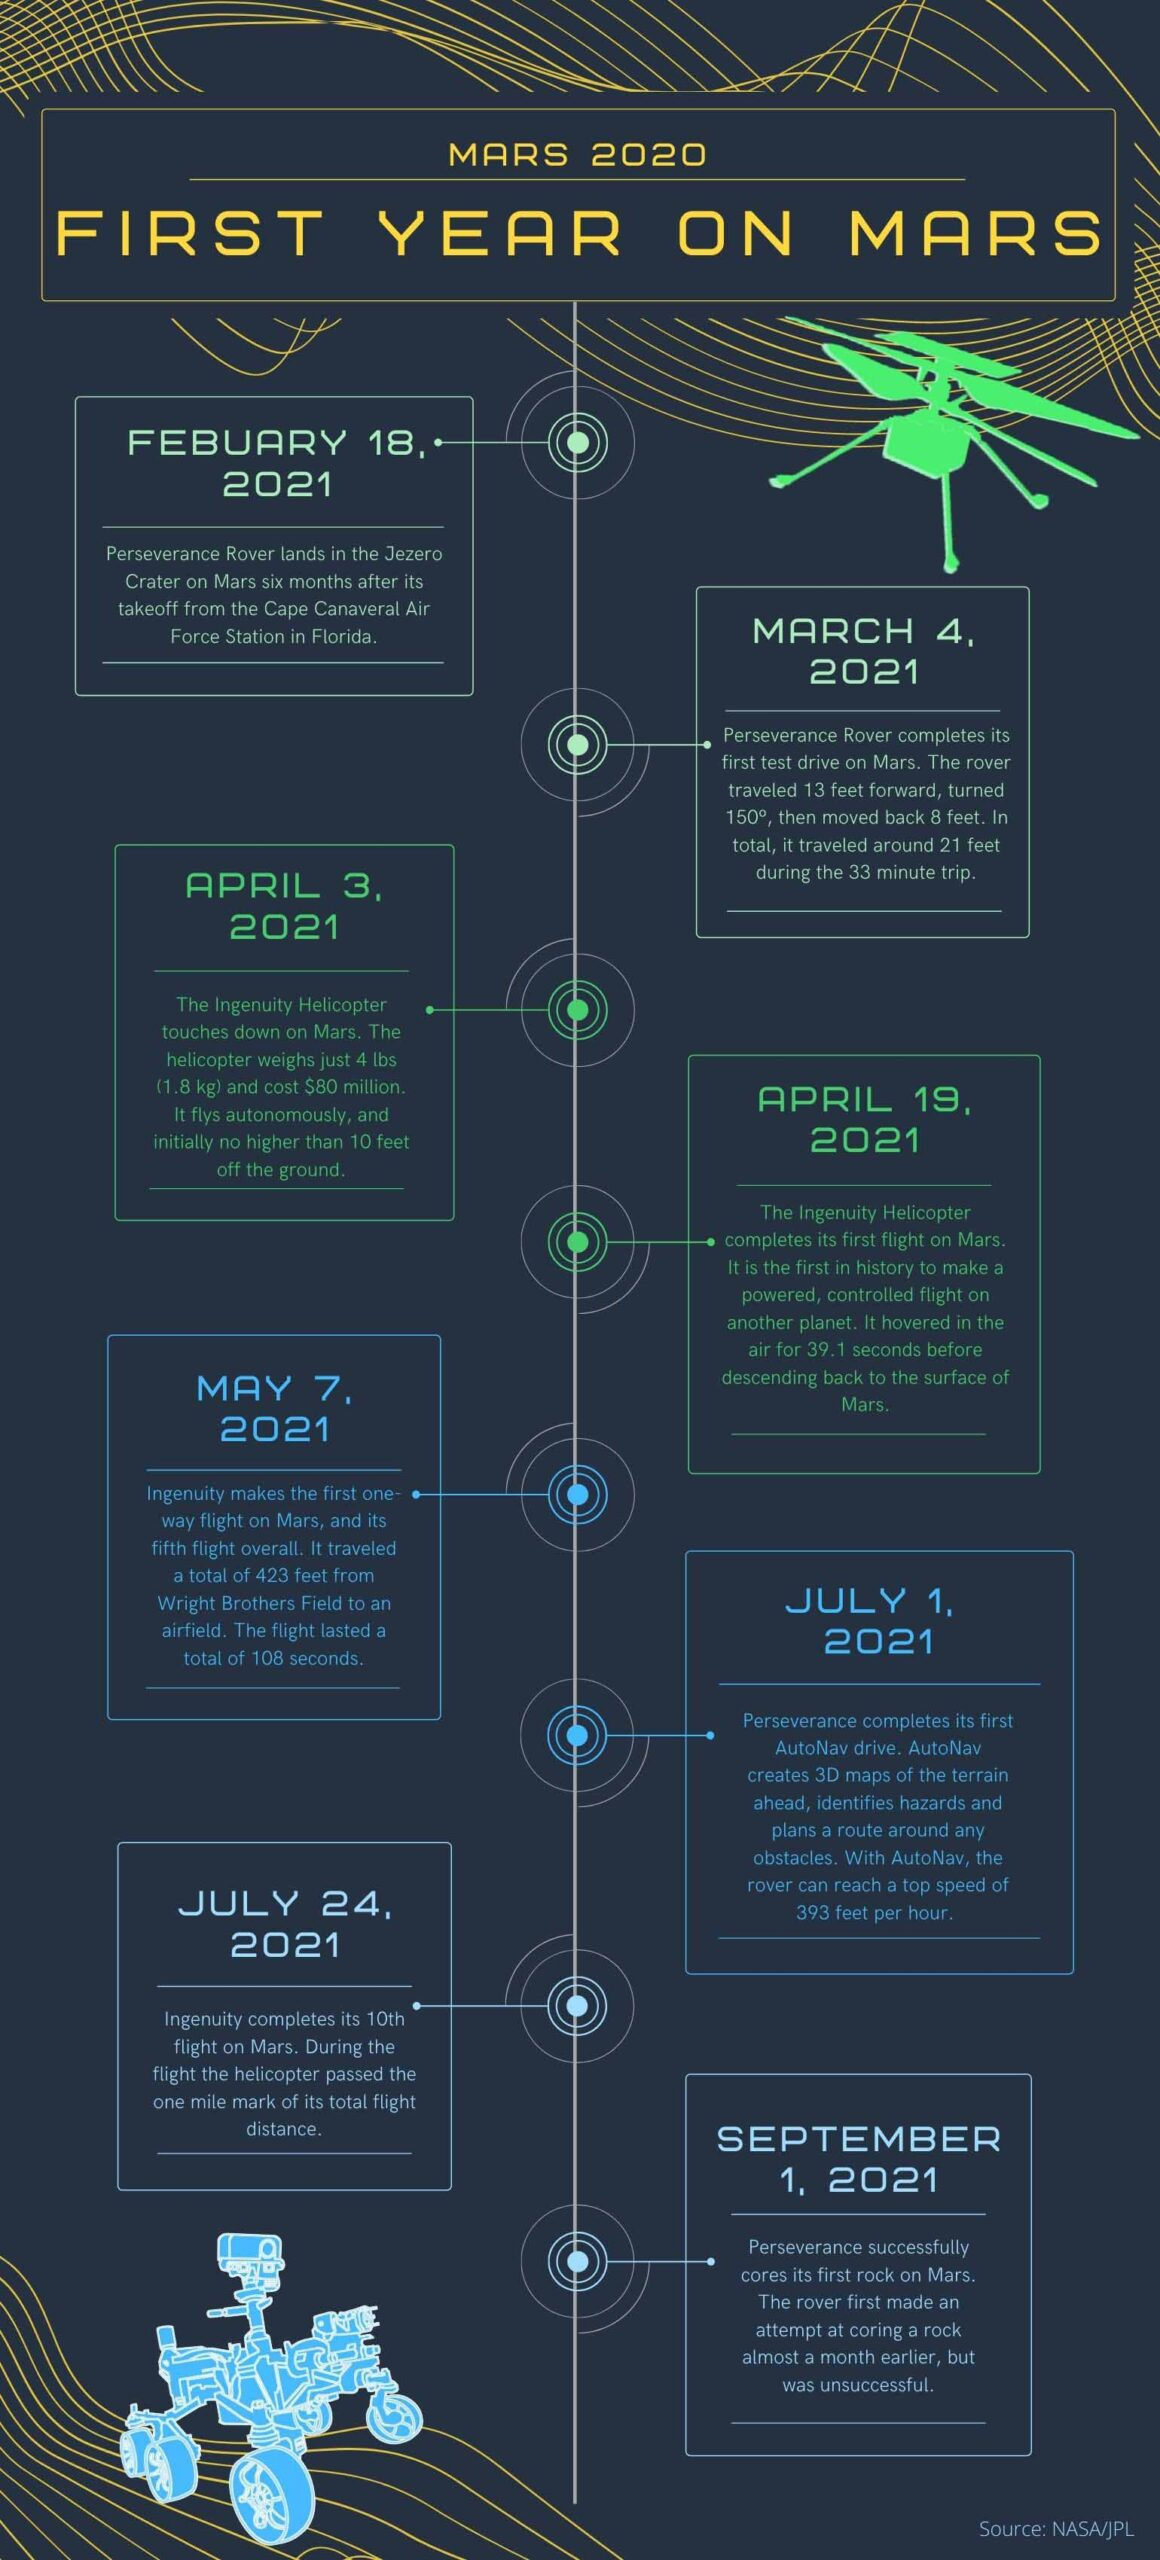
\includegraphics[width=\linewidth]{figures/First Year on Mars image.png}
    \captionof{figure}{Perseverance's first year on Mars. Credit: NASA/JPL-Caltech, via \textit{The Robot Report}~\cite{robot_report_year}.}
    \label{fig:first_year}
\end{minipage}%
\hfill
\begin{minipage}[t]{0.58\textwidth}
    \vspace{0pt}
    \begin{itemize}[leftmargin=*, topsep=0pt]
        \item \textbf{July 17 -- August 15, 2020} -- Launch window, when the positions of Earth and Mars were optimal for travel to Mars~\cite{mars2020_wiki}.
        \item \textbf{July 30, 2020, 11:50 UTC} -- Launch from Cape Canaveral Space Force Station, Florida~\cite{mars2020_wiki}.
        \item \textbf{July -- February 2021} -- Cruise phase; all trajectory correction maneuvers (TCM) successful, adjusting the spacecraft's course toward Mars~\cite{mars2020_wiki}.
        \item \textbf{February 18, 2021} -- Landing of \textit{Perseverance} on Mars surface~\cite{mars2020_wiki}.
        \item \textbf{March 4, 2021} -- First major test of \textit{Perseverance} drive functions~\cite{mars2020_wiki}.
        \item \textbf{April 3, 2021} -- Deployment of \textit{Ingenuity}~\cite{mars2020_wiki}.
        \item \textbf{April 3--4, 2021} -- MEDA recorded the first weather report on Mars~\cite{mars2020_wiki}.
        \item \textbf{April 19, 2021} -- First flight of \textit{Ingenuity}~\cite{mars2020_wiki}.
        \item \textbf{April 20, 2021} -- MOXIE generated 5.37\,g of oxygen from CO\textsubscript{2} on its first test~\cite{mars2020_wiki}.
        \item \textbf{June 1, 2021} -- \textit{Perseverance} begins its first science campaign~\cite{mars2020_wiki}.
        \item \textbf{July 5, 2021} -- Ninth \textit{Ingenuity} flight; first to scout areas inaccessible to the rover~\cite{mars2020_wiki}.
        \item \textbf{August 6, 2021} -- First sample acquired from the ancient lakebed~\cite{mars2020_wiki}.
        \item \textbf{May 3, 2022} -- Rover loses contact with \textit{Ingenuity} after 27 flights; contact restored after suspending science operations~\cite{mars2020_wiki}.
        \item \textbf{January 25, 2024} -- End of \textit{Ingenuity} mission after rotor blade damage on flight 72~\cite{mars2020_wiki}.
        \item \textbf{July 25, 2024} -- ``Leopard spots'' discovered on rock ``Cheyava Falls,'' with signs of possible ancient microbial life~\cite{mars2020_wiki}.
    \end{itemize}
\end{minipage}

\section*{Hardware Design}
Perseverance carries one of the most comprehensive sensor suites ever deployed on a planetary rover.
The Mastcam-Z provides high-resolution stereoscopic imaging and serves as the rover's primary
vision system, while the SuperCam instrument combines a laser, spectrometer, and microphone to
analyze rock composition at a distance~\cite{rover_components}. For close-up analysis, SHERLOC uses an ultraviolet
Raman spectrometer to detect organic compounds and biosignatures directly on rock
surfaces~\cite{rover_components}.

\begin{figure}[H]
    \centering
    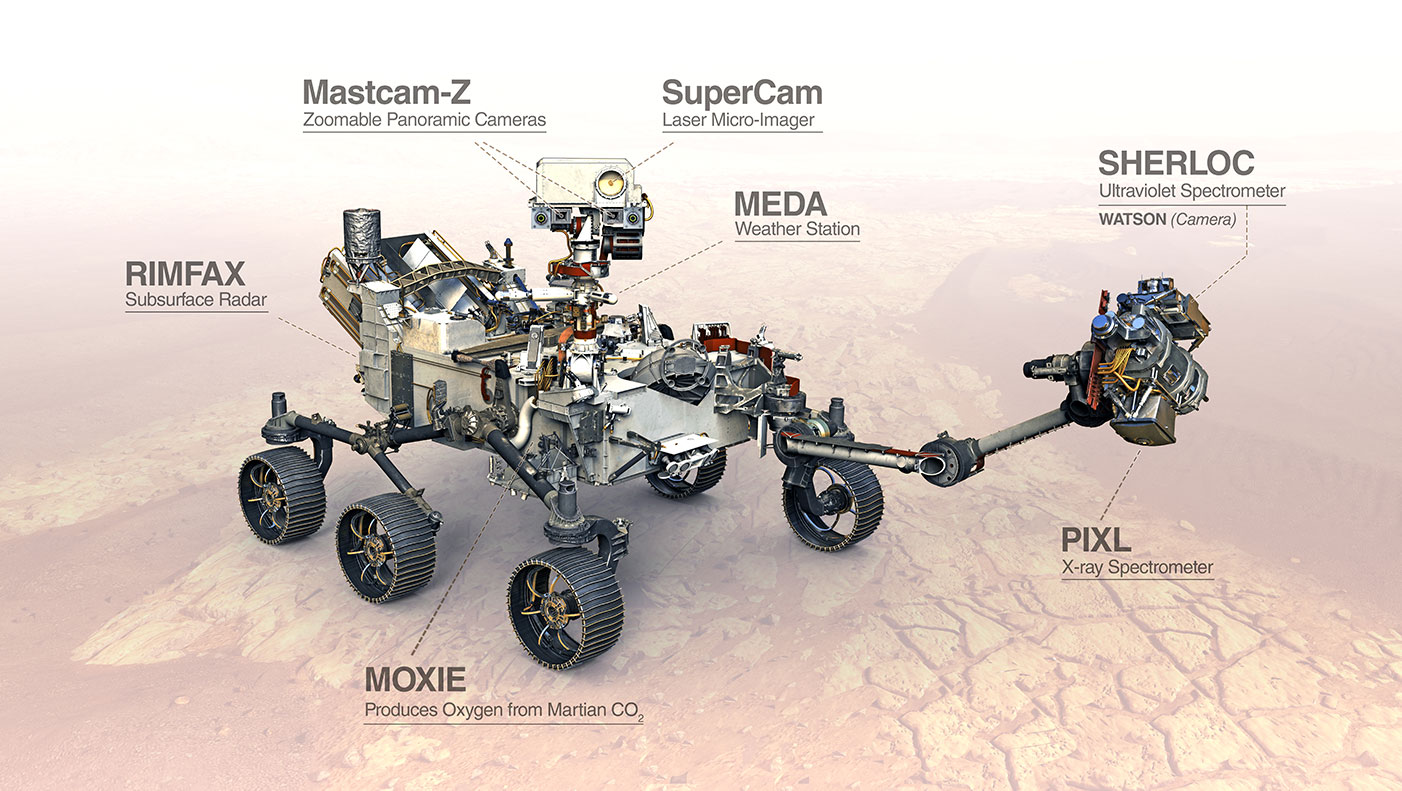
\includegraphics[width=0.9\textwidth]{figures/25045_Perseverance_Mars_Rover_Instrument_Labels-web_TJS8tKe.jpg}
    \caption{Diagram of the Perseverance Mars rover's science instruments. Credit: NASA/JPL-Caltech~\cite{jpl_teachable}.}
    \label{fig:perseverance_instruments}
\end{figure}

Navigation relies on a separate network of cameras (front and rear Hazcams paired
with NavCams) that feed into AutoNav's terrain modeling pipeline to identify obstacles in real
time~\cite{autonav_jpl}. The tight coupling between the science sensor suite and the navigation perception
hardware reflects a fundamental design constraint in robotics: sensing and autonomy
cannot be architected independently of one another.

\section*{Autonomous Capabilities}
A key challenge for automating the planetary rover is knowing where it is. Early in the mission, the rover
would capture a 360\textdegree{} panorama and a human operator would manually figure out its
position from a map of Mars~\cite{mgl_universetoday}. Advances in computer vision and localization now allow
Perseverance to determine its own position autonomously through a system called Mars Global
Localization (MGL)~\cite{mgl_universetoday}. This lets the rover operate 24/7 toward its goals
without waiting for Earth-based position confirmation~\cite{autonav_jpl}.

Perseverance is controlled by two processors operating in parallel, improving
fault tolerance and enabling multiple processes to run simultaneously~\cite{rover_components}. AutoNav holds the record
for the greatest distance driven by a Mars rover without human review: 699.9 meters in a single
drive~\cite{autonav_jpl,science_robotics}.

AutoNav functions as a hierarchical planner. Using MGL's localization output to establish its
position, it generates a 3D map of the surrounding terrain, identifies hazards, and computes a
route before executing it~\cite{autonav_jpl}. A local reactive layer runs alongside this global plan, allowing
the rover to respond to obstacles that appear between planning cycles. This two-layer architecture
is a well-established setup in robust robots, and Perseverance's consistent performance validates its use.

\section*{Outcomes \& Reflection}
I find the Perseverance mission particularly interesting because it embodies the idea of continuous
improvement: every mission should make the next design better. The wheel redesign was my favorite example of this.
Curiosity's aluminum wheels showed significant wear on Mars' sharp basalt rock,
so the Perseverance team redesigned the wheel with a thicker aluminum shell and a new tread pattern
to directly address that failure mode~\cite{rover_components}.

Perseverance goes beyond just being a tool for exploration. It is a demonstration of what integrated robotic
systems can achieve under extreme real-world constraints. Its autonomous localization stack, layered
control architecture, rich sensor arsenal, and durable mechanical design each reinforce the others,
forming a system that is more capable than any single subsystem could produce alone. As these
capabilities continue to advance in future missions, they help lay the groundwork for the human
exploration of Mars that ultimately depends on knowing the planet can be navigated by our machines first.

\newpage

\begin{thebibliography}{99}

\bibitem{mars2020_wiki}
Wikipedia contributors,
``Mars 2020,''
\textit{Wikipedia, The Free Encyclopedia}.
Available: \url{https://en.wikipedia.org/wiki/Mars_2020}

\bibitem{autonav_jpl}
NASA Jet Propulsion Laboratory,
``Autonomous Systems Help NASA's Perseverance Do More Science on Mars,''
\textit{NASA JPL News}, September 21, 2023.
Available: \url{https://www.jpl.nasa.gov/news/autonomous-systems-help-nasas-perseverance-do-more-science-on-mars/}

\bibitem{science_robotics}
V. Verma et al.,
``Autonomous robotics is driving Perseverance rover's progress on Mars,''
\textit{Science Robotics}, vol. 8, no. 80, p. eadi3099, July 26, 2023.
doi: \url{https://doi.org/10.1126/scirobotics.adi3099}

\bibitem{rover_components}
NASA Science,
``Perseverance Rover Components,''
\textit{NASA Science Mission Directorate}, July 22, 2025.
Available: \url{https://science.nasa.gov/mission/mars-2020-perseverance/rover-components/}

\bibitem{robot_report_year}
The Robot Report,
``A year of milestones for the Mars 2020 mission,''
\textit{The Robot Report}, February 18, 2022.
Available: \url{https://www.therobotreport.com/a-year-of-milestones-for-the-mars-2020-mission/}

\bibitem{jpl_teachable}
NASA Jet Propulsion Laboratory,
``Meet Perseverance: NASA's Newest Mars Rover,''
\textit{NASA JPL Education}, 2021.
Available: \url{https://www.jpl.nasa.gov/edu/resources/teachable-moment/meet-perseverance-nasas-newest-mars-rover/}

\bibitem{mgl_universetoday}
Universe Today,
``NASA's Techno-Wizardry Grants The Perseverance Rover Greater Autonomy,''
\textit{Universe Today}, February 20, 2026.
Available: \url{https://www.universetoday.com/articles/nasas-techno-wizardry-grants-the-perseverance-rover-greater-autonomy}

\end{thebibliography}

\vspace{1em}
\noindent\textit{\small Disclaimer: Claude Sonnet 4.6 (Anthropic) was used to compare this paper against the assignment rubric and provide a grade estimate.}

\end{document}
